\section{CMOS Scaling}
Since 1970 and until now, the number of transistors integrated with a single microprocessor has been continuously increasing.
In 2019 today, the CMOS scaling continues; the 5nm CMOS risk production is soon beginning and developments of the next CMOS node (3nm CMOS) are highly active \cite{3nm_imec}. For example, the TSMC 5nm node brings 15\% performance and 45\% area improvements compared to the 7nm node \cite{tsmc5nm}. 40 years ago, it has been said that the CMOS scaling limit is around 1um due to physical constraints (wavelength of light), but nearly 1000$\times$ of scaling is about to be accomplished with a number of technology breakthroughs.

While the motivation towards CMOS scaling can be diverse, it is largely driven by economic and financial reasons. 
That is, by utilizing further scaled CMOS process, the unit cost of a single transistor can be cut down and the chip performance can be improved by moving to advanced CMOS process nodes. Therefore, a chip with more competitiveness and higher profit margins can be manufactured, which is the most important factor in silicon business.
While CMOS fabrication companies (e.g. TSMC, Intel, Samsung, SMIC) invest an enormous amount of money and resource towards advanced CMOS processes and chip design companies invest largely on process porting, their expected ROI (return on investment) upon moving to the advanced nodes are much greater!

\subsection{Will CMOS scaling continue forever?}
The end of CMOS scaling will approach when the amount of investment overcomes the expected return, which is expected to be the 3nm node or the next \cite{itrs}. Then, what will happen to us circuit designers? Will we all lose our jobs?
A potential technological direction is: for a specific application, a dedicated process technology may be adapted. Let us return to the point that the CMOS process is dominantly used because of economic reasons (it is far cheaper than using other processes!), even though existing other dedicated process technologies perform better than CMOS.

However, that precondition will be broken with further scaling and when CMOS cost stops scaling. Strong motivation will be born to adapt non-CMOS process technologies. For example, for RF SoCs, a co-integration of CMOS and compound semiconductors (GaNs, SiCs) can become the mainstream. For mobile SoCs where power consumption is crucial, SoI CMOS may be used. Co-integrating silicon photonics and CMOS is an interesting technology \cite{issccphotonics1}, which may produce breakthroughs in wireline communications\cite{photonics1} and LiDARs \cite{photonics2}. 
These multi-device integrations are exciting directions and will bring design paradigms even to analog circuit designs.
Another optimistic technology direction is, the CMOS technology will cause a breakthrough (as it has done in the past decades) and process scaling will continue further on.

\subsection{Recent trends in CMOS scaling and digital circuits}
\begin{figure}[!]
\centering
  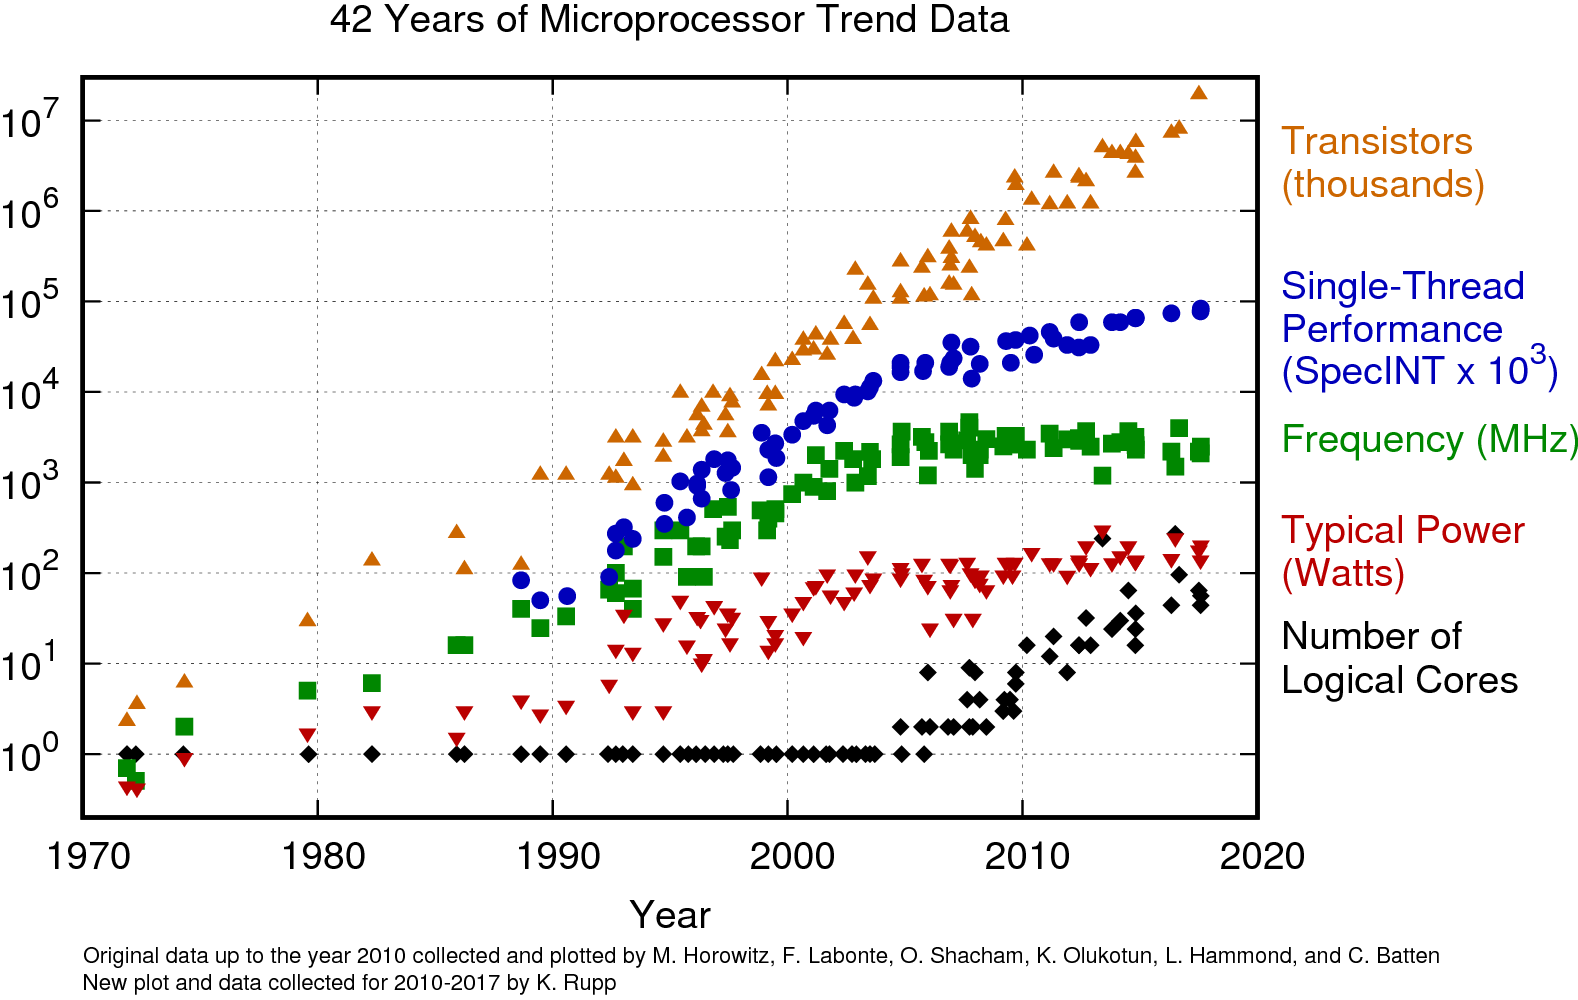
\includegraphics[width=1\textwidth]{figure/chap1/42-years-processor-trend.png}
  \caption{42 years of processor trend. (In courtesy of \cite{processor} \cite{danowitz2012cpu})}
  \label{cpu-trends}
\end{figure}

Let us return to the topic of the CMOS scaling trends.
Fig.\ref{cpu-trends} plots the processor performance of the last 42 years \cite{processor} \cite{danowitz2012cpu}.
While we say "scaling" in one word, the "Dennard's Law" scaling \cite{dennard1974design}, which keeps the power consumption of the chip constant, has already ended and "Moore's Law" scaling \cite{moore1965cramming} is the only one active, which simply increases the crammed number of transistors in a single chip.

When the "Dennard's Law" scaling was active, the device size and the clock frequency improved 30\% every process generation.
While this alone will explode the chip power, the entire power consumption of the chip was kept constant by scaling the power supply and the load capacitance.
Note that while the load capacitance benefits from the physical scaling effect, the power supply voltage was scaled down by lowering the transistor's threshold voltage.
However, "Dennard's Law" scaling ended around 2006 since the power supply voltage could no longer be turned down. Around this time, the transistor leak current (or off-currents) became a non-negligible power consumer in SoCs. Further scaling the transistor threshold voltage was difficult, since that will exponentially increase the leak currents.

After the Dennard scaling ended, the CMOS processors' performance becomes restricted by thermal density power (TDP) and not the clock speed. Chips cannot consume more power (or heat) than it can cool, or else the chip itself can be severely damaged if operated in high temperatures ($>$ 125 deg.).
One can notice the performance limitation by TDP when running a large program and monitoring the CPU clock rate; when the CPU temperature exceeds a certain amount, the CPU will configure to lower its clock rate, simultaneously degrading the processing performance. Thus, cooling technologies are highly active research areas in high-performance computing \cite{abci}.

Interestingly, the inconvenience that the "Dennard's Law" scaling has ended became a strong motivation towards developing new digital circuit technologies.
Conversely, when the Dennard scaling was active, the chip performance will greatly improve by just porting to a new process node; implementing new circuit technologies were not worth the try.
One technology direction where the digital architectures head is "general" towards "domain-specific".
For example, by looking at the number of logical cores in Fig. \ref{cpu-trends}, we can tell that processors are heading to increase the operation parallelism and functionalities. 
While it is difficult to improve the performance of general single-instruction operations, multi-core processors boost the performance of highly-parallel operations and multi-task programs.
Graphic processing units (GPUs) architectures evolved extremely in this direction. State-of-the-art GPU has over 8000 cores \cite{v100} and has become the \textit{de facto} standard for graphic processing and deep neural network training. While each core is simple compared to x86 cores, the enormous amount of parallelism becomes highly effective in "domain-specific" tasks like vector/matrix/tensor processing.

\begin{figure}[!]
\centering
  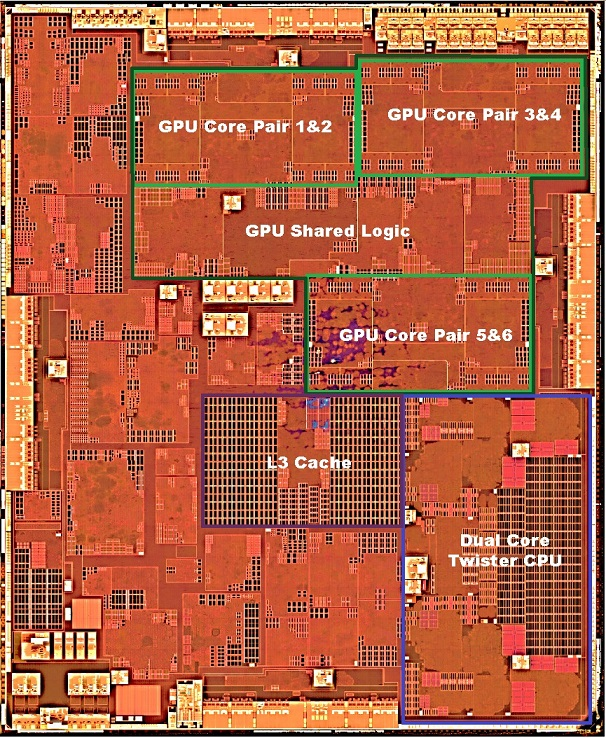
\includegraphics[width=0.8\textwidth]{figure/chap1/A9PNG.jpg}
  \caption{Apple A9 chip. (In courtesy of \cite{a9})}
  \label{A9}
\end{figure}

A number of processors utilize specialized hardware, given the extra number of transistors to be used.
For example, smartphones have a very strict power budget and its processor power efficiency is top of mind.
The iPhone A9 processor (Fig.\ref{A9}) has a dedicated CPU and GPU but also over 50 "specialized hardware" exist to process images, video, audio signals and to ensure extra user-security.
Such "specialized hardware" can only perform a dedicated operation (e.g. encode video) but its power efficiency is extremely high compared to general processors.
Moreover, dynamic voltage and frequency scaling (DVFS) techniques have become common in mobile SoCs to extremely scale power when the workload is small.
To conclude, while performance improvements for general processors have hit the wall, "domain-specific" hardware has given rise. 
Interestingly, it can be interpreted economically that the investment return on architectures and technologies is now higher than investment in process technologies.

\subsection{Process scaling (and problems) with analog circuits}
\begin{figure}[!]
\centering
  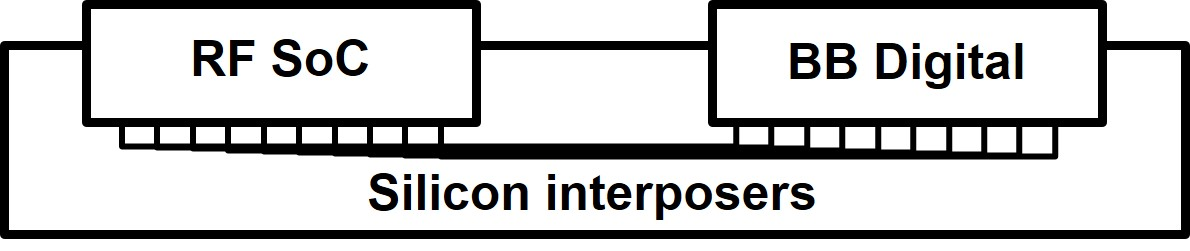
\includegraphics[width=0.8\textwidth]{figure/chap1/interposer.jpg}
  \caption{Modern RF SiP integration}
  \label{RFSIP}
\end{figure}

Here, we will explain the analog circuit evolution trend in the last decade, compared to digital circuits.
However, the largest problem in analog circuit design is that commonly, analog circuit performance degrades when moving to advanced nodes.
We will study this effect further in the following sections.
Generally, when we move to an advanced CMOS process node, we see that the analog circuit area scaling is much smaller than that of digital circuits.
Therefore, the relative cost of analog circuits (per unit area) becomes higher and higher.

For some time, this impact on the SoC cost was neglected by the large cost scaling of digital circuits. 
However, the cost scaling of digital circuits has also become slower; it is becoming challenging to accept the increasing costs of analog circuits.
In the latest smartphones (iPhone XS Max and Galaxy X released in 2018) \cite{iphoneXS} \cite{galaxy}, the RF analog circuits and baseband digital circuits are separated to different chips.
While splitting chips causes additional integration costs, we can infer that even with such integration costs, it has become more cost-efficient to get rid of analog circuits from the baseband digital chip.


However, applications such as mobile communications and high-speed IOs, which heavily utilize analog circuits, demand exponential performance improvement per product generation. To keep up with the pace of the performance improvements, the analog circuits must scale its area and performance as well.

\begin{figure}[!]
\centering
  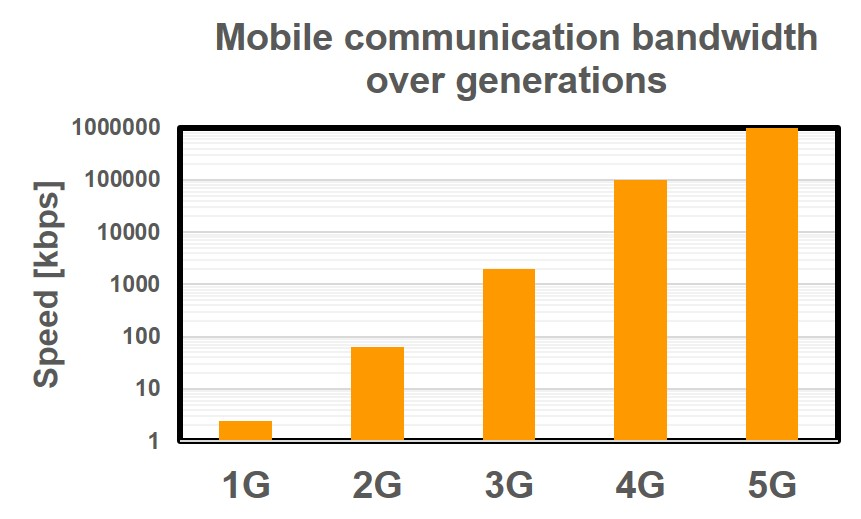
\includegraphics[width=0.8\textwidth]{figure/chap1/wireless-trends.jpg}
  \caption{Wireless performance trends}
  \label{wireless-trends}
\end{figure}

Fig. \ref{wireless-trends} shows the performance trend of mobile communication provided by the Third Generation Partnership Project (3GPP) \cite{3gpp}. During the 1G-2G-era, the communication speed was only a few kbps, which restricted the mobile phone applications to text data transferring. However, as it approached the 3G era, the maximum communication speed reached up to a few Mbps and opened up various mobile applications such as images, audio, and games. When the communication standards reached LTE and 4G, the speed evolved exponentially as well and opened up possibilities to even playing high-quality movie data via streaming. Nowadays, the 5G experimental services are beginning and its communication speed and capacity will evolve every year as well, even trying to reach a communication bandwidth of 100 Gbps \cite{sasaki2018experiment}. 5G is seeking emerging applications given its excellent performance and potentials; for example, streaming all of the automobile's sensor data via 5G to realize a fully-autonomous vehicle controlled by cloud servers \cite{autonomous}.

To further extend the evolution of wireless standards, high-performance analog circuitry are inevitable. Since mobile devices can not scale the battery capacity, the total hardware power consumption should score a par even with faster communication speeds. Otherwise, the mobile device battery life will degrade every time the wireless generation advances. To achieve this goal, the wireless circuit performance must track the CMOS scaling trends as well. Therefore, not only digital circuits but the analog circuitry must also scale its power efficiency along with CMOS process scaling; CMOS process scalable analog circuits are in high demand.

%Commonly, such modern wireless modules (like smartphones) implement analog RF ICs (RF circuits and baseband ADCs) with relatively legacy CMOS process (e.g. 28nm CMOS). On the other hand, baseband digital ICs (or modems) are integrated with cutting-edge nodes (e.g. 7nm CMOS) \cite{galaxy}. Then, such chips can be integrated with silicon interposers and ship as a single package (Fig.\ref{RFSIP}). However, wireless communication trends try to boost up the communication capacity as the standards evolve (e.g. 5G, 6G..), even trying to reach a communication bandwidth of 100Gbps \cite{sasaki2018experiment}. Moreover, the industry heads towards to increase the number of multi-input and multi-output (MIMO) and carrier aggregations (CA). Thus, the number of analog transceiver circuits must scale with the MIMO and CA; if the analog CMOS process is fixed, scaling the number of analog circuits will directly impact the chip cost, making the realization of the future wireless trends extremely challenging.

The analog circuits failing to scale are not a problem for wireless devices. For example, inter-processor and inter-server communication commonly utilize high-speed I/O circuits with ADC based receivers \cite{wireline} \cite{wireline2}.
CPU-GPU communication is done by PCIe busses and in the next generation (Gen.6 a.k.a PCIe 6.0), the PCIe standard requires PAM-4 based TX/RX to achieve 64 Gbps communication \cite{PCIe}.
PAM-4 communications require high-performance ADCs and DACs operating at over 10 GS/s, which will largely dominate the IO performance and cost. Since CPU-GPU communication uses a 16$\times$ link, at least 16 sets of ADCs are required in the IO circuitry. The ADC cost and performance must be extensively scaled to realize such a high-performance IO.
While ADC-based transceivers have not been adapted for DRAM memory IOs yet, it may be replaced in the future if the bandwidth requirements continue to grow.


\begin{figure}[!]
\centering
  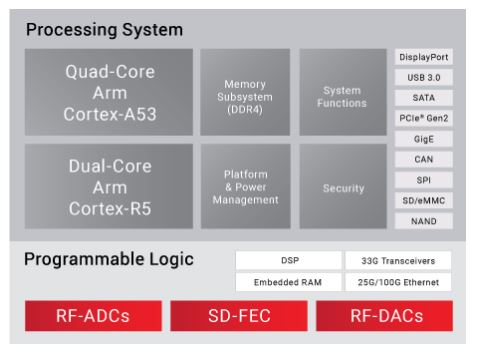
\includegraphics[width=0.8\textwidth]{figure/chap1/fpga.JPG}
  \caption{FPGA with analog circuit integration (In courtesy of \cite{fpga})}
  \label{FPGA}
\end{figure}

For a long time, ADC industrial researches were long driven by companies such as Analog Devices and Texas Instruments. However, such companies do not have a strong motivation to tackle into analog designs with advanced technology nodes because their main products are discreet analog devices and legacy nodes play along well.
Recently, Xilinx drives researches of scaled CMOS analog circuits for high-speed I/Os and software-defined radios. Recent publications include $>$ 4GS/s 13-bit ADCs in 16nm FinFET \cite{xilinxadc} \cite{xilinxadc2} and integrated high-speed ADC based IOs \cite{xilinxwireline}.

By integrating the ADCs with the 16nm node, such circuits can be integrated within the FPGA (ZYNQ UltraScale + RF SoC is shown in Fig.\ref{FPGA} \cite{fpga}). 
For baseband stations with excessive numbers of MIMO, FPGAs integrated with multiple channels of high-performance ADCs can lower the system bill of materials (BOM) cost and power consumption, compared to the legacy implementation which integrates multiple discrete ADC chips.

\subsection{Analog circuits' scaling effect}
Similar to digital circuits, can we take the analog circuit's scaling challenges as a step to revolutionize analog circuit designs?
This thesis aims to establish an analog circuit design technique which is CMOS process scalable, especially focused on Nyquist ADCs.
Before going to the details, we would like to study why analog circuits cannot compete with CMOS process scaling.

Here, we will focus on an operational amplifier circuit (Opamp), which is the key analog design components for multiple circuits (e.g. switched capacitor circuits, amplifiers, and filters).
While there are multiple performance figures for an Opamp we will focus especially on: Gain-Bandwidth (GBW which couples with speed), output amplitude swings (which couples with noise), and lastly, gain (which couples with precision). To start, we will study the effect of scaling on each of the analog circuit performance measures.
First of all, GBW improves with process scaling. Since the transistor GBW is decided by: 
\begin{equation}
GBW = g_m / C_p
\end{equation}
the parasitic capacitor $C_p$ shrinks with scaling and GBW improves.
On the other hand, the output swing is affected by the decreased power supply voltage. 
Therefore, it is essentially impossible to improve the output swing and is damaged by scaling. If the power supply decrease 10\% by moving to an advanced node, relatively the analog circuit output swing, and noise performance will decrease \textit{at least} 10\%.

Finally, we discuss the scaling effects to gain performance. 
The opamp gain is the most important factor upon obtaining high accuracy in pipeline ADCs. 
The adverse effects of scaling are most apparent in gain performance and are affected by both supply voltage drop and transistor analog performance degradation. 
Commonly, there are three approaches to achieve high-gain in Opamp design: 1.) cascode the transistors, 2.) increase the transistor W/L size to increase $g_m$, and lastly, 3.) increase the number of Opamp stages.
A cascode configuration requires a voltage headroom of $2 V_{od} + 2 V_{th}$, the rest of the voltage margin is assigned to the output amplitude. 
However, let us expect $V_{th} = 0.4 V$, $V_{od} = 0.1 V$ and power supply voltage 0.9V in 28 nm CMOS technology.
Critically, with cascoding, the voltage headroom alone reaches 1V, exceeding the power supply voltage! 
Therefore, cascode connection cannot be utilized under low power supply voltage. 
While Opamp gain can be enhanced by increasing $g_m$ and the number of stages, such approaches consume much more power than cascoding.

Another problem in scaled CMOS analog circuit design is the degraded performance of the transistor itself.
As well known, with a sufficiently large output resistor, the gain of a common source amplifier circuit can be derived as 
\begin{equation}
  Gain = g_m \times r_o    
\end{equation}
where $r_o$ is the output resistance of the transistor. While $r_o$ directly couples to gain, the value of $r_o$ is an inverse proportion to the channel length ($L$) and utilizing scaled transistors will damage the Opamp gain.
While we can obtain sustainable $r_o$ by venturing the use of large $L$, this approach cannot gain any benefits from process scaling; the relative cost of analog circuits will eventually increase.

\section{Towards process scalable analog circuits}
\begin{figure}[!]
\centering
  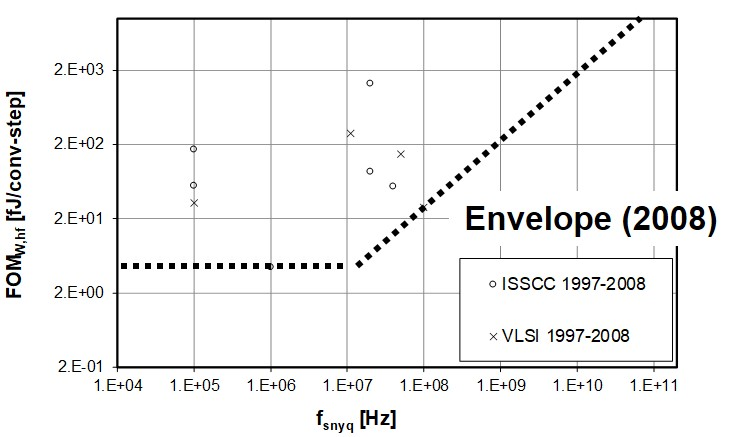
\includegraphics[width=0.8\textwidth]{figure/chap1/sar-performance-2008.jpg}
  \caption{SAR ADCs published in ISSCC, VLSI (1997-2008)}
  \label{sar2008}
\end{figure}

\subsection{Rise of SAR ADCs}
On the other hand, there also exists an analog circuit whose performance improves by process scaling. 
A typical example is the SAR ADC.
Conventionally, SAR ADCs were utilized for low speed, high-resolution ADCs due to their nature which requires multiple successive approximation (SA) cycles to complete the conversion. 
Typically, the number of required SA cycles is equivalent to the number of state bits. 
On the other hand, Pipelined and Flash ADC's conversion time is overwhelmingly short and have been adapted for high-speed applications. 
For example, in the case of Flash, the conversion delay is similar to that of a single comparator delay. The pipeline ADC's conversion delay consists only of a sub-ADC conversion and signal amplification, naturally suiting high-speed applications. 
However, all circuit blocks of the SAR ADC benefit from scaling and its performance have improved along with CMOS scaling.
Due to that fact, the SAR ADC's performance improvement over the last decade was remarkable and looking back at the history of published SAR ADCs in the last two decades is very informative.

Fig.\ref{sar2008} plots the SAR ADC performance published in ISSCC and VLSI during 1997-2008, whose data are based on \cite{MurmanADC}.
The x-axis shows the sampling speed and the y-axis shows the Walden figure of merit (FoM) \cite{walden1999analog}.
During those days, the most advanced process node was 65nm CMOS and most of the works were based on 130nm or 180nm CMOS.
To plot the evolution of unit-SAR ADC performances, we exclude time-interleaved ADCs in the plot, whose fastest unit SAR ADC was 100MS/s.
The Elzakker SAR ADC \cite{elzakker} was presented at ISSCC 2008 (is included in the plot), which improved the SAR ADC power efficiency by $10\times$ (!) compared to the prior art. This work showed one shape of an "accomplished" SAR ADC, which gave rise to extensive researches upon further improving the SAR ADC performance and is still active until now.

\begin{figure}[!]
\centering
  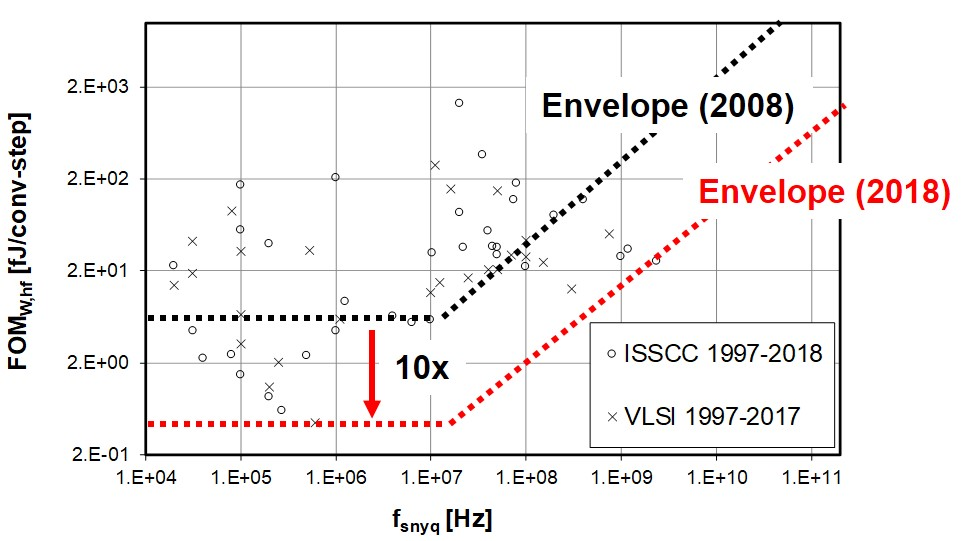
\includegraphics[width=0.8\textwidth]{figure/chap1/sar-performance-2018.jpg}
  \caption{SAR ADCs published in ISSCC, VLSI (1997-2018)}
  \label{sar2018}
\end{figure}

Fig. \ref{sar2018} shows the SAR ADC performance presented during ISSCC and VLSI until now (1997-2018) \cite{MurmanADC}.
Firstly, the process technologies evolved greatly in the past ten years, and the most advanced node presented was 14nm CMOS.

Let us study the evolution in both terms of speed and power efficiency.
The SAR ADC research direction splits into mainly two paths: those that pursue power efficiency at low speeds ($<$ 1MS/s) and those that pursue high-speed, high-resolution performance aiming to replace Pipelined ADCs. 
For the former, the power efficiency was further pushed and reached even 0.4fJ/conv., mainly due to the optimization (supply voltage were reduced from 1V to 0.3V, which improves the energy efficiency $10\times$) and improved process nodes.
Therefore, the SAR ADC energy bounds were pushed nearly 10$\times$ in the past 10 years, which are beneficial to  realize low-powered and high-precision sensor devices for IoT systems.
Interestingly, many SAR ADCs that achieve $>$ 10-bit and high-speeds ($>$ 100MS/s) have also been published and is an active research area.
Since $>$ 100MS/s ADCs are mandatory for mobile communications (LTE and WiFi), power-efficient SAR ADCs replacing the power-hungry Pipelined ADCs are in high demand.
The speed boundaries have also been pushed 10$\times$, which greatly expanded the application of SAR ADCs.

\begin{figure}[!]
\centering
  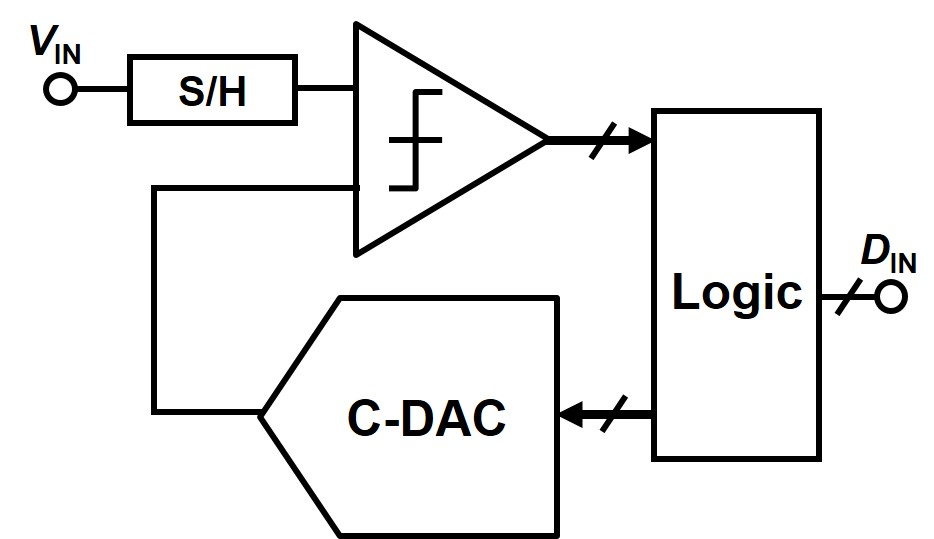
\includegraphics[width=0.8\textwidth]{figure/chap1/ch1-sar-block.jpg}
  \caption{SAR ADC circuit block diagram.}
  \label{sarblock}
\end{figure}

Before going into the further details of the SAR ADC, the fundamental SAR ADC operation is explained briefly.
The block diagram of the $n$-bit SAR ADC is shown in Fig. \ref{sarblock}.
After sampling the input signal $V_{in}$, the comparator compares either the input or the reference voltage is larger.
The reference voltage utilized during the comparison is generated by the C-DAC, which has a resolution of $n$-bit as well.
Since C-DAC is the only analog (in terms of having multiple voltage levels) component in the ADC, the ADC linearity is determined by this circuit.
The comparison result is stored in the logic circuit, and the reference voltage is shifted in the direction in which the input range can be narrowed down.
The SAR ADC operation is binary search: during the initial comparison (or MSB cycle), the SAR ADC configures if the input signal is larger than 1/2 $V_{ref}$ or not. 
If the input signal is smaller, the reference voltage will be shifted to 1/4 $V_{ref}$ and if larger, the reference voltage will be configured to 3/4 $V_{ref}$.
The procedure above is one cycle, and by repeating for the given number of cycles, fine analog-to-digital conversion results are obtained. 

Next, we will review the function of each circuit in the SAR ADC and consider the impact of process scaling.
Fundamentally, the SAR ADC cycle time can be represented by the sum of the delays of the comparator, logic, and C-DAC, as shown bellow.
\begin{equation}
     Cycle = t_{Comp} + t_{Logic} + t_{CDAC}
\end{equation}
First of all, the process scaling effect appears most straightforwardly in logic circuit delays.
Since the SAR ADC's logic circuit is mainly composed of flip-flops, the delay of the logic is almost equivalent to the digital gate delay. 
Therefore, similar to a general digital circuit's scaling effect, the delay will be 30\% faster for every time the process node advance.

Also, comparators benefit from scaling and the speed will improve proportionally to the GBW and digital gate delay. 
In general, the comparator circuit can be divided into two circuits, a preamplifier circuit that converts the voltage difference between two inputs into a current difference, and a latch circuit that will amplify the current difference and output as a digital value. The delay of the latch circuit corresponds to the digital gate delay, similar to $t_{Logic}$. 
The speed of the preamplifier circuit corresponds to the transistor GBW, which also improves with process scaling.

Also, $t_{DAC}$ is proportional to the unit capacitance of the C-DAC. In legacy process technologies, capacitors were created by inserting insulators between vertical metal layers (metal-insulator-metal MIM capacitor). While MIM capacitor has a superior matching property, the minimum capacitance is quite large (10-50fF).
On the other hand, advanced process technologies enable the use of metal-oxide-metal (MOM) capacitors, which simply utilize the parasitic capacitance born between metals. Since the metal fabrication accuracy has improved significantly, it has become possible to create highly accurate capacitors. 
Because MOM capacitors can utilize very small unit capacitance (down to 500aF), the energy consumption and the delay of the C-DAC has greatly improved together with developments of efficient C-DAC switching techniques \cite{ccliu-sar-adc}.

\subsection{Fundamental Problems of the SAR ADC}
Although the SAR ADC has made a performance breakthrough in the past decade, the performance enhancement has hit a brick wall. We will study this further in this section. As a rule-of-thumb, realizing a high-resolution and high-speed SAR ADC is challenging. In this section, we will analyze some fundamental reasons behind this.

One of the challenges which SAR ADCs face is the reference voltage settling constraints. 
Due to the structure of the binary C-DAC, when the large MSB capacitor is switched after the first comparison, a large amount of charging/discharging occurs. 
Such sudden charge fluctuation causes ringing in the reference voltage, because of the LC resonance of the bonding inductance. 
To obtain high accuracy by the SAR ADC, such voltage ringing must be attenuated within $<$ LSB/2 to LSB/4, since fluctuated reference voltage corrupts the conversion accuracy. 
Since a typical solution is to simply "wait" until the ringing calms down, this prolongs $t_{C-DAC}$ and limits the conversion speed.

One way to reduce the voltage ringing is to utilize a large "decoupling" capacitor on-chip so that sufficient amount of charge can be supplied on-chip.
However, such decoupling capacitors can easily reach few nFs \cite{zhou201512} \cite{verbruggen201470} to achieve high-accuracy.
Such capacitors can be even several times larger than the ADC core, and its cost overhead may not be acceptable for low-cost mobile SoC applications.

Another way to get around the voltage settling is by providing an on-chip voltage buffer.
With a sufficient buffer bandwidth, we can suppress reference voltage fluctuations.
On the other hand, this breaks the premise that SAR ADCs do not require an active element; voltage buffers are a high-bandwidth power-hungry opamp.
While the power consumption of the voltage buffer is typically excluded in the ADC performance presented at academic conferences, some works report that the utilized voltage buffer itself consumes 4$\times$ more power than the SAR ADC itself \cite{ccliu201612}. 
If the SAR ADC included the voltage buffer in its core area, most high-speed high-resolution SAR ADCs may even under-perform the power efficiency of state-of-the-art Pipelined ADCs.

\section{Hybrid ADCs}
As mentioned in the previous section, it is fundamentally difficult to realize a high-resolution and high-speed SAR ADC.
On the other hand, Pipelined and Flash ADCs alternatives but do not meet the power efficiency requirements of mobile devices.
Therefore, to overcome this challenge, there has been extensive researches to make use of the SAR ADC in other ADC architectures, 
often called "Hybrid" ADCs, which is an ADC architecture that fuses two different ADCs (e.g. Pipelined ADC and SAR ADC).
By utilizing a Hybrid ADC architecture, designers can accomplish performances that were difficult with "Monolithic" ADCs.

\subsection{Pipelined-SAR ADCs}
Here, we will study deeper on "Pipelined-SAR ADCs", which are one of the most successful Hybrid ADCs to date.

While we say "Pipelined ADCs are power-hungry", why is that?
One of the major reasons is that Pipelined ADC requires \textit{multiple} power-hungry Opamps (and amplification circuitry), depending on the number of Pipelined stages.
Therefore, Pipelined-SAR ADC aims to lower the power consumption by minimizing the number of Pipeline stages by utilizing a SAR ADC as the high-resolution Quantizer \cite{lee2011sar2stagepipeline} \cite{furuta201110}.
Conventionally, Flash ADCs were utilized as the Quantizer but its resolution was limited to 4-bit since the required number of comparators must increase exponentially with resolution. By replacing the Flash ADC to a SAR ADC, the quantizer resolution can be greatly improved over the limits ($>$ 6-bits). While such configuration impacts the conversion speed, since SAR ADCs are much slower, this can be countered in deep scaled CMOS where the SAR ADC conversion speed improves.

The Pipelined-SAR ADC in \cite{lee2011sar2stagepipeline} uses a two-stage configuration of 6-bit 1st stage SAR + 6-bit 2nd stage SAR to construct a 12-bit ADC in total.
The residue voltage generated in the 1st stage SAR ADC is amplified 64 $\times$ and sampled via the 2nd stage SAR, realizing a two-stage operation.
Since only one residue amplifier is required, the overhead of pipelining is minimized and high power efficiency can be obtained.

Moreover, Pipelined-SAR ADC holds several merits over the SAR ADC as well.
Firstly, the conversion speed excels. Pipelined-SAR ADCs require only 6 SA cycles and amplification during the conversion cycle, in contrary to the 12-bit SAR ADC which requires 12 SA cycles.
Besides, since the conversion is performed in two-steps, the reference voltage settling requirements are greatly relaxed. 
Specifically, if there is 0.5-bit redundancy between stages, the reference voltage requirement of each stage is only the 1/4 of the 6-bit LSB (which is equivalent to 16 LSB for full 12-bit resolution). Compared to 12-bit SAR ADCs which require the reference to settle within 1/4 of the 12-bit LSB, the design of reference buffers or decoupling capacitors is significantly relaxed, which will contribute to reducing the total system cost.
Thus, the hybrid architecture combining pipeline and SAR ADCs can enjoy the advantages of both architectures and achieve both high performance and high power efficiency.

\subsection{Design challenges of the Pipelined-SAR ADC}
However, even though Pipelined-SAR ADCs achieve high performance, significant design challenges remain.

1.) \textbf{Pipelined-SAR ADCs requires high precision residual amplification.}
For such amplification, a high-gain opamp is indispensable but such designs are difficult to realize in scaled CMOS process.
While various approaches have been taken to realize high-gain amplifiers in scaled CMOS (detailed benchmarks will be done in Chapter 2), none have been able to completely overcome the analog process scaling challenges.

2.) \textbf{Most designs utilize complex digital gain calibrations.} Hence, many designs utilize digital calibration to counter the gain error and tolerate the use of a low-gain amplifier. Since precise gain is not required, this approach allows the use of power-efficient open-loop (or dynamic) amplifiers \cite{zhou201512} \cite{verbruggen201470}. However, sudden supply voltage variations cannot be tracked and suppressing such fluctuations with bypass capacitors significantly impacts chip cost. While environment variation tracking dynamic amplifiers have been proposed, start-up calibration is still necessary \cite{pvt-dynamicamp}. Such gain-calibrations are very complex, which typically takes several tens of ms and requires additional analog circuits as well. Such calibration overheads are further discussed in chapter 2.

To conclude, while Hybrid ADCs achieved a breakthrough in performance, it is not a silver bullet towards process scalability and several critical design challenges remain.

\section{Thesis motivation and organization}

\begin{figure}[!]
\centering
  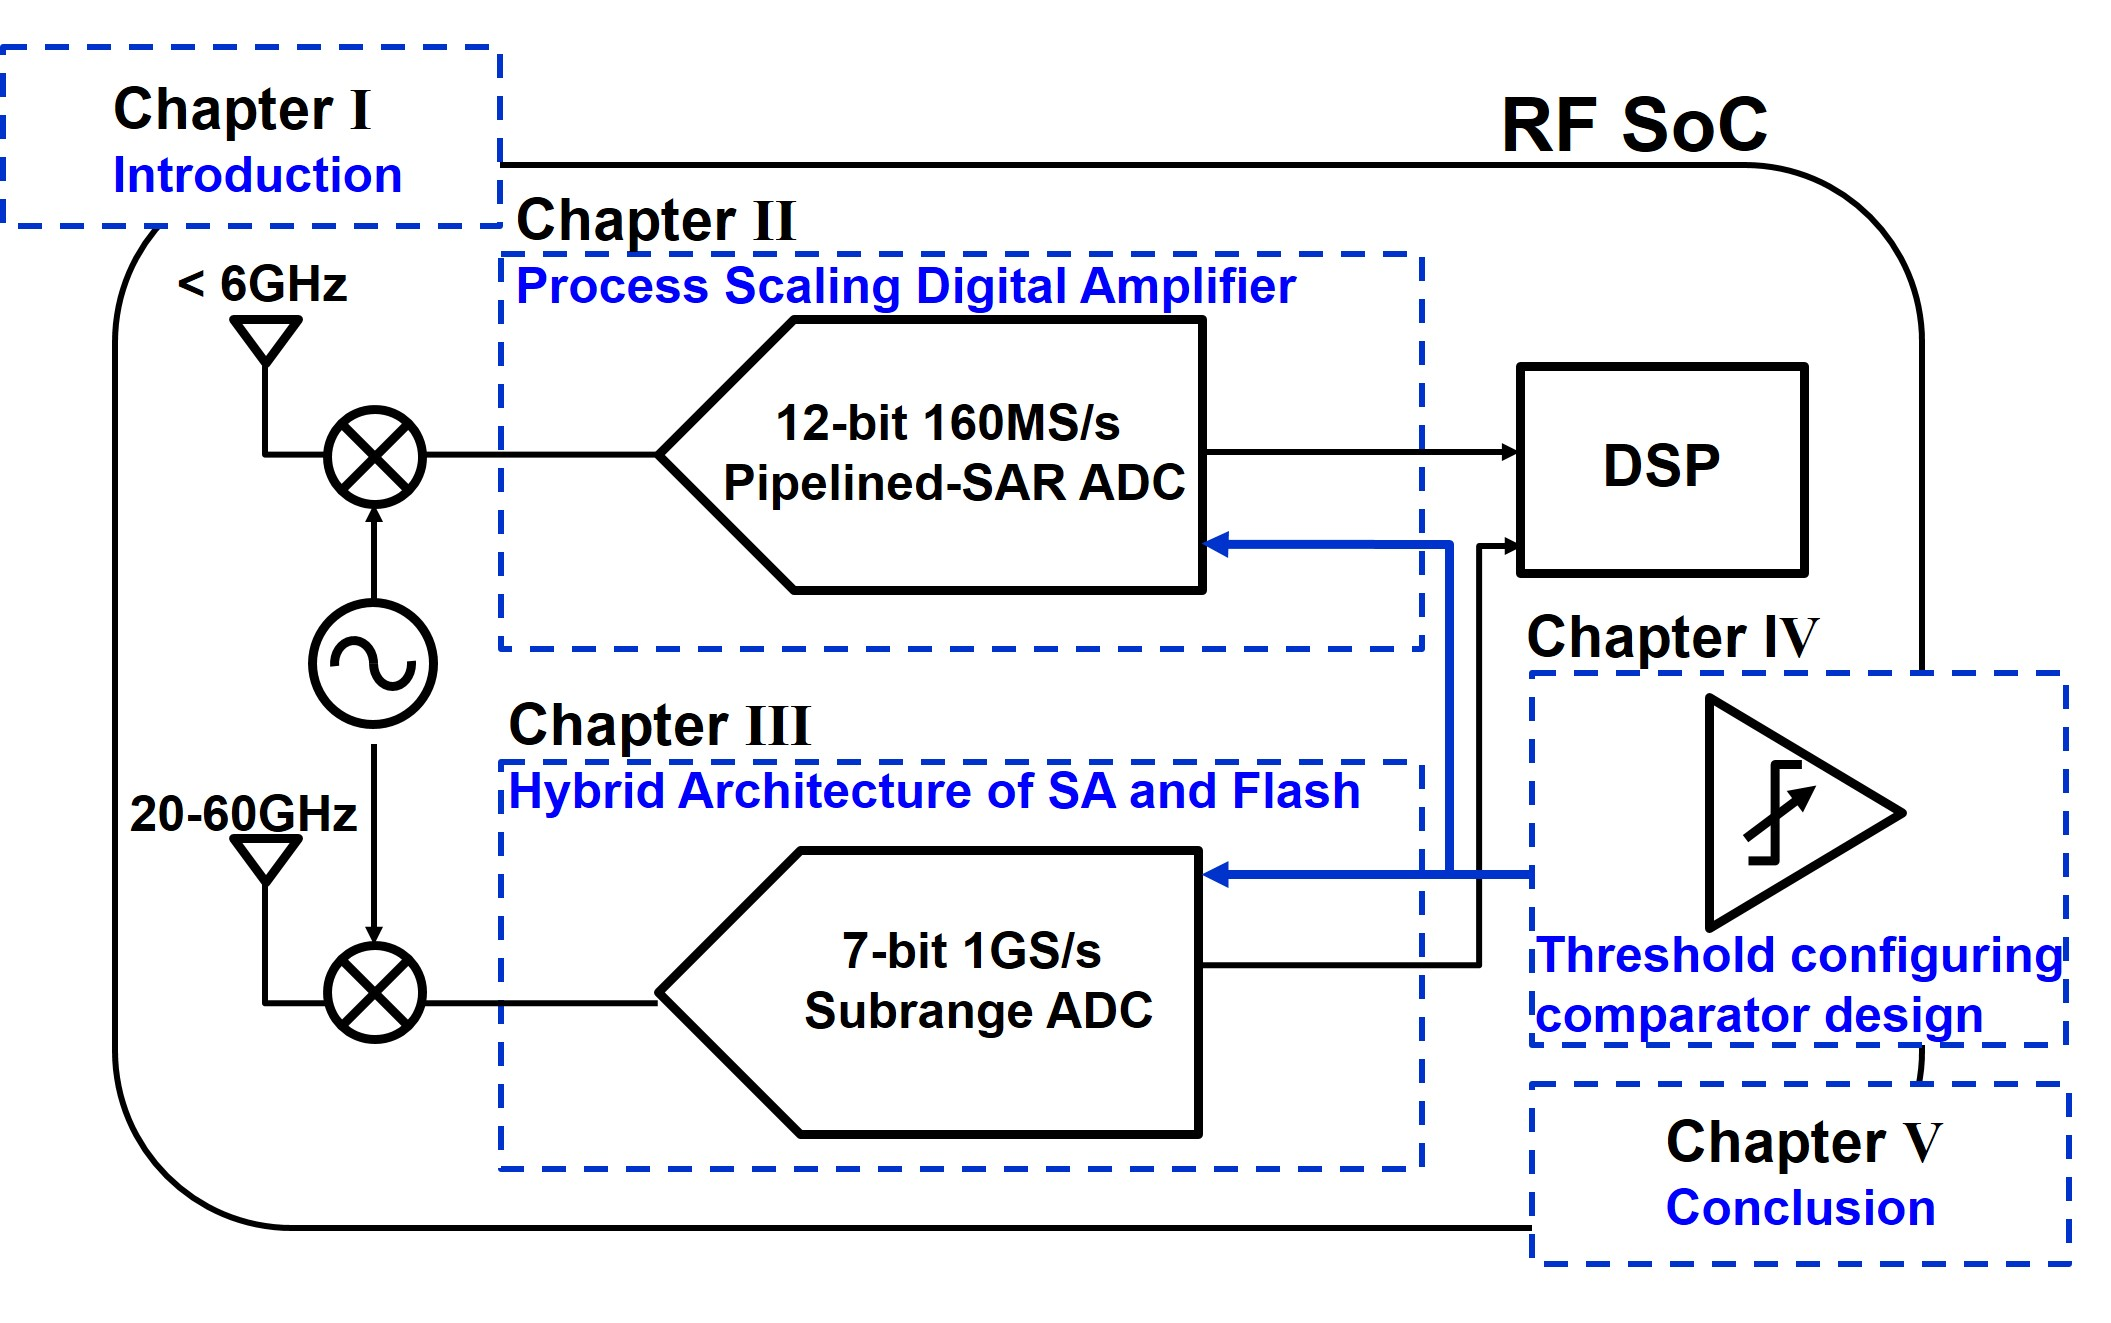
\includegraphics[width=1\textwidth]{figure/chap1/thesis-org.jpg}
  \caption{Thesis organization.}
  \label{thesis-top}
\end{figure}

In this thesis, design techniques towards CMOS process scalable and power-efficient Nyquist ADCs are explored. 
Our thesis construction is shown in Fig.\ref{thesis-top}.
The key approach we take upon realizing a process scalable ADC is: \textbf{1) aggressively utilize the scalable successive approximation (SA) circuitry} and \textbf{2) propel a Hybrid with the existing ADC architectures.}
 
We target the ADC application to wireless baseband ADCs for mobile devices in this thesis.
Modern wireless standards  (e.g. 802.11ax WiFi \cite{11ax} and 5G \cite{andrews2014will}) feature mainly two frequency bands: an under 6GHz band for long distance communications and $>$ 20GHz ultra-wide band for extremely-high-speed communications \cite{802.11ad} \cite{rappaport2013millimeter}, typically called as ultra-wideband (UWB) communications.
Thus, at least two types of baseband ADCs will be required to realize such modern wireless systems. And most importantly, such ADCs are required to be power-efficient as possible, since the battery life of mobile devices is one of the largest concerns. 

\begin{figure}[!]
\centering
  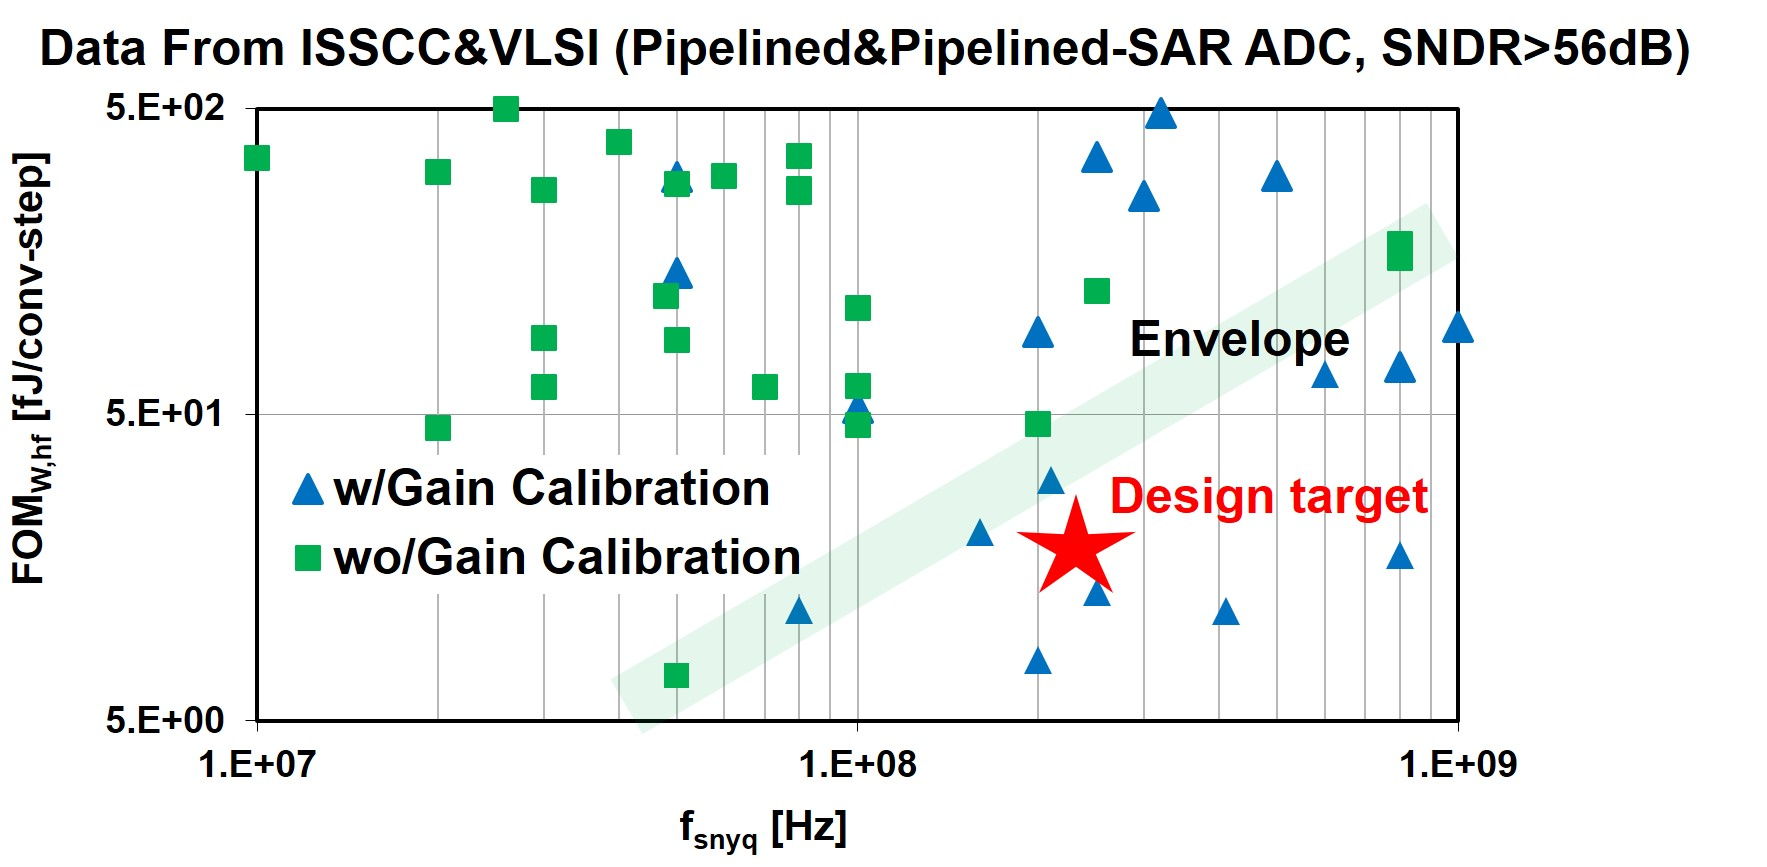
\includegraphics[width=1\textwidth]{figure/chap1/target.jpg}
  \caption{Benchmark for high-speed high-resolution Pipelined ADCs.}
  \label{target}
\end{figure}

\textbf{1) We target our first ADC for $<$ 6GHz wireless communication, which is required to be medium-speed and high-resolution.}
Since the baseband bandwidth can be as large as 80MHz, we target the ADC speed to 160MS/s.
To establish communications even with long distances (several km), the ADC must sufficiently convert input signal with very small amplitudes.
Therefore, for such applications, we target the ADC resolution to 12-bit (effective SNDR of 60dB).
Since this ADC is most frequently used for wireless communications, high power efficiency is required to prolong battery life; we target the ADC power efficiency to 20fJ/conv., which is state-of-the-art performance.

Such high-performance is difficult to achieve with a monolithic SAR ADC, given its performance limitations. Therefore, Pipelined-SAR architectures will be the best candidate, but a large design challenge remains when realizing a high-precision amplifier in a scaled CMOS process (e.g. 28nm CMOS). We benchmark such ADCs in Fig. \ref{target}, where we plot the published Pipelined-SAR and Pipelined ADCs. Due to the design challenges, most of the works achieving high power-efficiencies utilize complex digital calibration to relax the amplifier design requirements (plots in blue triangles). Moreover, such designs pose problems in PVT variations and PSNR (power supply versus noise ratio), which can become troublesome during system integration. 
On the other hand, works without gain calibration have far worsened power-efficiencies (over 3 $\times$ worse) and do not meet the demand for mobile devices.  Thus, our design target is to design a high-performance Pipelined-SAR ADCs without the need for digital calibrations in deep-scaled CMOS process.

\textbf{2) We target our second ADC for $>$ 20GHz ultra-wideband (UWB) communications, which is required to be high-speed and low-precision.}
Even with mobile devices, there is a large demand to deliver large-capacity contents like videos and movies. To deliver such contents with high-quality, a UWB communication that is fast as wireline communications are demanded. 
The baseband frequencies of such UWB communications can reach up to several GHz. In this thesis, we target our ADC speed to 1GS/s and plan to time-interleave such unit ADCs to reach higher speeds, if demanded.
In UWBs, the distance between the base station and the carrier will be very close (several tens of meters) and the received signal level is considered to be relatively high. Thus, we set the ADC resolution to 7-bit (SNDR 35dB).
While such ADCs are common for applications like measurement instruments and wireline communications  \cite{kullveryfastsar}, such ADCs are very power-hungry and does not meet the demands of mobile devices. Therefore, low-power and high-speed ADC design techniques are in high demand.

\subsection{Thesis organization}
Here, we will briefly discuss the organization of the thesis.
\\
\\
In chapter 2, design techniques for process scalable Pipelined-SAR ADCs are explored.
We focus especially on the switched-capacitor amplification circuit, which becomes the largest obstacle when implementing Pipelined-SAR ADCs in scaled CMOS processes.
To tackle the problem that Opamp gain cannot be obtained in scaled processes, we propose the Digital Amplifier (DA) technique to realize power-efficient and accurate amplification in scaled CMOS. 
DA cancels out all errors (i.e. gain error, non-linearity, settling, and thermal noise) of the low-gain Opamp by feedback based on successive approximation (SA).
Moreover, the DA accuracy can be arbitrary set by configuring the number of bits in the DA C-DAC; the amplifier gain is decoupled from the transistor analog performance which brings in a new design paradigm and the design methodologies for DA is deeply discussed. Interestingly, since the majority of the amplification is "digital" operation, due to the nature of SA circuitry, the DA circuit is highly process-scalable.

To confirm the power-efficiency of the DA, we implemented a 0.7V 12-bit 160MS/s Pipelined-SAR ADC in deeply scaled 28nm CMOS, which meets our target for $<$ 6 GHz baseband ADCs.
The Pipelined-SAR ADC does not require any digital gain calibration and achieves SNDR=61.1dB, FoM=12.8fJ/conv.. The ADC accomplished a world's best power-efficiency (over 3$\times$ improvement) compared to conventionally published calibration-free high-speed pipelined ADCs. In addition, we evaluate the DA’s process scalability by comparing the measured results of the DA-based MDAC prototyped in 65nm and 28nm CMOS. We observe 2-3$\times$ improvement in speed, power, and area mainly resulting from the DA’s process scalability.
\\
\\
In chapter 3, we explore power-efficient and process scalable ultra-high-speed ADCs, required for high-capacity wireless communications.
While conventional Flash ADCs achieve a very fast conversion rate, its power consumption is notorious.
Moreover, while the ADC sampling rate varies dynamically in wireless systems (because the number of available channels varies with environment), Flash ADCs will always consume high-power irrespective of the sampling rate. Digital circuits realize super-linear power scaling by dynamically scaling the power supply voltage reflecting the CPU clock frequency \cite{DVFS}, but high-speed ADCs are very sensitive to power supply variations; dynamically scaling the supplies are not realistic.

To achieve super-linear power scaling in high-speed ADCs, we propose to dynamically configure the ADC \textit{architecture} reflecting the ADC clock frequency which we name Dynamic Architecture and Frequency Scaling (DAFS).
The ADC architecture is reconfigured between successive-approximation and flash every clock cycle, relying on the conversion delay. 
To realize architecture configuring with small overheads, successive-approximation/flash reconfigurable ADC is proposed, which just adds few gates to conventional successive-approximation (or binary search) ADCs. 
The DAFS operation is fully automatic; the flash operation is adaptively performed by detecting excess delays during conversion and no pre-programming is required. 
We also show that DAFS not only significantly improves the power scaling but also compensates for transistor speed shifts due to process, voltage and temperature (PVT) variations as well.

A prototype subranging ADC is fabricated in 65 nm CMOS, which operates up to 1220MS/s and achieves SNDR of 36.2dB. 
DAFS is active between 820–1220MS/s and achieves peak power reduction of 30\%, when compared with the power scaling when DAFS is disabled. 
A peak FoM of 85fJ/conv. was obtained at 820MS/s, which is 2x more power efficient than reported subranging ADCs, at the time the paper was presented.
\\
\\
The ADC techniques presented in chapters 2 and 3 heavily rely on comparator performance.
For example, the amplification speed of the DA in chapter 2 is largely dominated by the successive approximation (SA) cycle time. 
If the number of SA cycles can be reduced by multi-bit conversions, the ADC conversion speed can be greatly improved but such multi-bit conversions require variable threshold comparators.
Moreover, if the comparators can hold a variable threshold voltage, the binary-search ADC utilized in chapter 3 can get rid of reference generation circuits which consumes a non-negligible amount of static power.

In chapter 4, we aim to design threshold configurable comparators (TCC) to improve the performance of successive approximation based circuits.
Such TCCs are benefitable, but has a number of design issues: 1) is difficult to implement if the threshold configuring range is very large. 2) TCCs typically have low power-supply-noise-rejection (PSNR), and the threshold can easily drift with even small supply fluctuations.

We propose current source based TCCs to enable wide-range threshold configurability. 
Moreover, we propose simple $V_{cm}$ biased current sources, which maintains sufficient comparator PSNR and keeps the ADC free from power supply variations over 10\%. 
To prove the effectiveness of the TCC, we implement a 2-bit/step SAR ADC where the 2-bit/step comparison is carried out by TCCs instead of area and power-consuming C-DACs.
The prototype ADC fabricated in a 40nm CMOS achieved a 44.3dB SNDR with 6.14MS/s at a single supply voltage of 0.5V, and achieves a peak FoM of 4.8fJ/conv-step.
\\
\\
Finally, in chapter 5, we summarize the thesis and establish a conclusion.
